% !TEX root = ./docs.tex

\author{Jan Grübener, Patrick Mischka}
\subsection{Grafische Benutzeroberfläche}

Bei dem Start eines Clients kann der Nutzer zwischen einem Commandline-Interface oder einer GUI wählen.
In der GUI wird der Nutzer aufgefordert sich mittels Nutzernamen und Passwort zu identifizieren. Wenn dies erfolgreich war wird dem Nutzer eine Übersicht seiner Chats angezeigt.
Am oberen Seitenbeginn ist der eigene Nutzername angezeigt, daneben ist ein Plus-Symbol, mit dem neue Chats erzeugt werden können. 
Hierbei gibt der Nutzer den neuen Chatnamen ein, als auch die Anzahl der zusätzlichen Chatteilnehmer. Folgend müssen die konkreten Chatteilnehmer genannt werden. 
Damit ein neuer Chat erstellt werden kann, müssen alle beteiligten Nutzer eingeloggt sein, damit der Schlüsselaustausch für die Verschlüsselung stattfinden kann.
Ist das erfüllt, wird der Chat erstellt und der Nutzer gelangt wieder auf die Chatübersicht. Wenn mindestens einer der Nutzer nicht eingeloggt ist, wird dies dem Nutzer angezeigt. Er kann dann entweder erneut versuchen den Chat zu erstellen oder navigiert mithilfe des Pfeil-Icons zurück in die Chatübersicht.
Durch Anklicken eines Chats in der Chatübersicht, wird der konkrete Chat geöffnet. Hierbei werden alle Nachrichten des Chats angezeigt. Am unteren Ende der Seite ist ein Texteingabefeld, mit dem der Nutzer auch Nachrichten in den Chat schreiben kann. Diese werden entweder durch eine Enter-Eingabe oder das Anklicken des Flugzeug-Icons verschickt. Nachrichten werden mit dem Nutzernamen des Erstellers für andere Nutzer angezeigt. 
Neben dem Chatnamen ist ein Pfeil-Icons, mithilfew dessen der Chat wieder geschlossen werden kann und sich wieder die Chat-Übersicht öffnet.

\author{Jan Grübener, Patrick Mischka}
\subsection{Verwendung von Emojis}

Bei der Verwendung von Emojis haben wir auf Unicode-Zeichen zurückgegriffen. 
Wir wollten die Nutzung von Icons als Bilddateien und den damit verbundenen Netzwerkverkehr und benötigten Speicherplatz so weit wie möglich vermeiden.
Neben dem Texteingabefeld eines Chat ist ein Icon, das beim Anklicken eine Übersicht über die verwendbaren Emojis öffnet und diese bei erneutem klicken auch wieder schließt. 
Die Emojis in der Übersicht können angeklickt werden, damit sie in Form eines Unicode-Zeichens an die aktuelle Stelle im Texteingabefeld übernommen werden.
\\ \\
Über die Implementierung wird im Codewalkthrough eingegangen.

//TODO wie ist eigentlich unsere Impl
\author{Matthias Vonend, Aaron Schweig, Troy Keßler}
\subsection{Gruppenchats}
Die bestehende Chatimplementierung ermöglicht Gruppenchats ohne weitere Anpassungen. Konversationen zwischen zwei Nutzern stellen einen Gruppenchat mit lediglich zwei Teilnehmern dar.
Wird eine Nachricht empfangen, werden diese an alle am Chat beteiligten Nutzer gesendet.

\author{Matthias Vonend, Troy Keßler}
\subsection{Mehrere Chatverläufe pro Nutzer}
Mehrere Chatverläufe sind eine Erweiterung der bestehenden Chatimplementierung. Nun ist es möglich mehrere Chats zu erstellen und zwischen diesen zu wechseln.
Im Client können die Chats eines Nutzers mit dem Befehl \textit{/chats} angezeigt werden. 
Mit dem Befehl \textit{/openchat} kann er dann diese Chats öffenund gelangt dabei in die Chatansicht wo er sowohl Nachrichten empfangen als auch senden kann.
Mit dem Befehl \textit{/quit} kann er die Chatansicht wieder verlassen und einen anderen Chat öffnen.

\author{Matthias Vonend}
\subsection{Persistentes Speichern der Chatverläufe}\label{persistance}
Sämtliche der Node bekannten Informationen (Nutzer, Chats, Nachrichten) werden in einem Warehouse verwaltet. 
Um diese Informationen zwischen Node-Neustarts zu persistieren, muss das Warehouse als Datei gespeichert werden. 
Bei einem Node-Start wird das Warehouse wieder geladen. Existiert noch kein Speicherstand, wird die Node mit einem leeren Warehouse initialisiert.
Während die Node ausgefallen war, können andere Nodes neue Informationen erhalten haben. 
Sobald die Node wieder verfügbar ist, müssen andere Nodes dies bemerken und die ausgefallene Node mit Informationen versorgen. 

Der Speichervorgang kann je nach System und Warehousegröße länger dauern. 
In dieser Zeit können in der Regel keine weiteren Anfragen verarbeitet werden. 
Um keine eingehenden Anfragen zu blockieren, kümmert sich ein eigener Thread um die Speicherung des Warehouses.
Bricht eine Node während des Speichervorgangs zusammen würde die Node sämtliche Informationen verlieren, da die Speicherdatei korrupt ist.
Um dies zu verhindern wird der Speicherstand zunächst in eine Tempdatei geschrieben und nach erfolgreicher Speicherung an den Zielort verschoben.

\author{Troy Keßler, Michael Angermeier}
\subsection{Verschlüsselte Übertragung der Chat-Nachrichten}\label{encryption}
Um einen sicheren Nachrichtenkanal zu gewährleisten, ist eine Ende-zu-Ende-Verschlüsselung implementiert. 
Beim Erstellen eines Chats wird ein Schlüssel mithilfe des Diffie-Hellman-Key-Exchange unter allen Teilnehmern generiert.
Dieser Schlüssel wird im Client mit der korrespondieren Chat-Id gespeichert, sodass verschlüsselte Nachrichten
auch nach einem Neustart des Clients wieder gelesen werden können. Dies ist notwendig, da auf dem Server nur die verschlüsselten
Nachrichten gespeichert sind und sonst keinerlei Möglichkeit bestehen würde, diese wiederherzustellen. 

Die öffentlich bekannte Primzahl, sowie die Generatorprimzahl wurden dabei für jeden Client festgeschrieben.
Nach jedem Login und nach Erstellen eines Chats generiert der Client einen neuen 128bit Schlüssel und löscht den alten, um die Sicherheit zu erhöhen.
Um auch Gruppenchats ermöglichen zu können musste der Diffie-Hellman-Key-Exchange entsprechend erweitert werden.
Dabei gibt es in Gruppen im Gegensatz zu zwei Teilnehmern mehrere Runden.
Ein Schlüsselaustausch mit drei Teilnehmern kann aus \hyperref[DHKE]{dieser Abbildung} entnommen werden.

\begin{figure}[h]
  \centering
  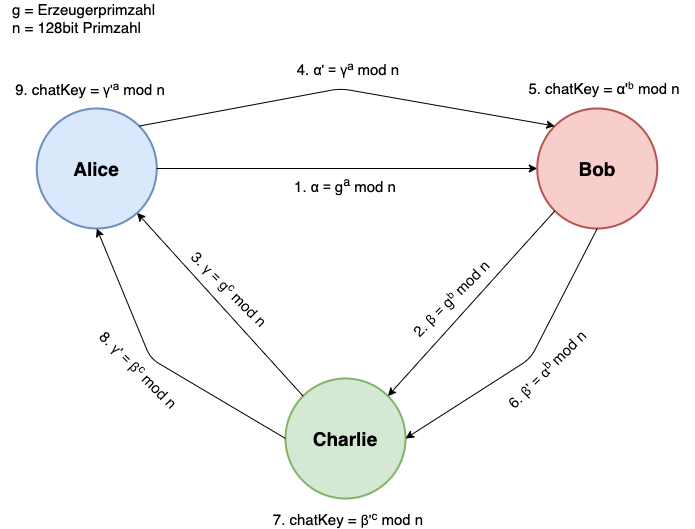
\includegraphics[width=\textwidth]{dh.png}
  
  \caption{Erweiterter Diffie-Hellman}
  \label{DHKE}
\end{figure}

Wie man erkennen kann werden in der ersten Runde (Schritte 1-3) die ersten Teilschlüssel wie im klassischen Diffie-Hellman generiert und weitergeschickt.
In der zweiten Runde werden mithilfe der Ergebnisse der ersten Runde, die fertigen Chat-Schlüssel berechnet (Schritte 4-9).
Die Größe der Primzahl n beträgt 128bit und die Länge der Generatorprimzahl 32bit. Die Schlüssellänge beträgt ebenfalls 128bit.

Dieses Verfahren kann mit beliebig vielen Teilnehmern durchgeführt werden, 
jedoch steigt die Anzahl der Runden linear und die Anzahl der Requests quadratisch.

Sei $n$ die Anzahl der Teilnehmer, so gilt:
\[
\begin{split}
  rounds &= n - 1\\
  requests &= n \cdot (n - 1)  
\end{split}
\]
Nachdem alle Chatteilnehmer den finalen Schlüssel berechnet haben kann der Chat erstellt werden. Dies ist der Fall,
wenn die Bedingung $$ currentRequests = (targetRequests - userIndex) $$ erfüllt ist, wobei $targetRequests$ die theoretische Anzahl
an Requests die gesendet werden müssen darstellt, mit $$targetRequests = n \cdot (n-1).$$
Die Variable $currentRequests$ beschreibt, wie oft das Paket schon weitergeleitet wurde.
Der $userIndex$ steht für die aktuelle Position im Schlüsselaustausch. Dabei ist der Initiator, mit einem Index von 0, der Erste.
Im obigen Beispiel mit drei Teilnehmern wäre also die Endbedingung erfüllt, wenn der Initiator ein Paket erhält, 
welches sechs mal weitergeleitet wurde.
$$ 6 = (3 * (3 - 1)) - 0 $$
%Aus Implementierungssicht braucht der Initiator dieses Schlüsselaustauschs eine Endbedingung, sodass er nachdem
%die Schlüssel unter allen Teilnehmern ausgetauscht wurden den Chat erstellen kann. Der Initiator dieses Schlüsselaustauschs 
%kann nun mit der Bedingung

% prüfen, ob der Schlüsselaustausch vollständig durchgeführt wurde.


Für alle anderen Clients gilt eine leicht abgeänderte Endbedingung. // TODO Welche, Brah?

Da nun alle Chatteilnehmer den gleichen Schlüssel besitzen und der Chat erstellt ist, können Nachrichten mit 
einem symmetrischen Verfahren sicher versendet werden. Hierfür wird die AES-Verschlüsselung verwendet.

\author{Troy Keßler}
\subsection{Verschlüsselte serverseitige Speicherung der Chats}
Durch die in \ref{encryption} beschriebene Ende-zu-Ende Verschlüsselung liegen dem Server die Nachrichten \textbf{nie} als Klartext vor.
Wie bereits in \ref{persistance} erwähnt werden alle Nachrichten im Warehouse gespeichert und das gesamte Warehouse wird abgespeichert.
So liegen auch in der Speicherdatei die Nachrichten niemals als Klartext vor.
